% ============================================================
% ch01_02.tex —— 第 1 章「基本群」 + 第 2 章「覆叠空间」
% 印刷 pp.3–20（PDF p43–p60，共 18 页；其中 p.12、p.20 为空白页）
% 底本：Springer LNM 2386, Ch.1 The Fundamental Group / Ch.2 Covering spaces
% 本块无编号公式（tags2.txt 中该页段为空，已核对图像）
% ============================================================

\chapter{基本群}
% [原文 p.3]

\ChapterAbstract{在代数拓扑中，人们关注用代数方法研究拓扑空间的性质。两个拓扑空间若同胚，便被视为“相同”，而适当的拓扑不变量可用来区分不同胚的空间。这类不变量中最主要的是同调群与同伦群。同调是一种对拓扑流形的洞与边界分支进行计数的工具；它在数学的许多分支中以非常核心的方式出现，在物理中亦然，例如 [72] 所开创的超对称弦论紧化。另一方面，同伦也刻画拓扑空间，但它考察的是空间上的道路而非其边界。同伦群中最简单的是第一同伦群，也称拓扑空间的基本群。本章是对若干标准拓扑概念的基础而细致的介绍，这些概念对于理解谱网络的构造十分重要。在给出一些基本概念之后，我们引入基本群并考察它的若干基本性质，以及若干把基本拓扑空间在同胚意义下区分开来的应用。关于本章所述主题的进一步资料，极佳的入门读物是 Hatcher 的教材 [192]（网上可免费获取），以及 [109]、[264] 与 [277]。}

\section{商拓扑}

拓扑学研究的是在具有连续逆的连续映射下的形状。改变拓扑的一个重要操作是粘合操作。这一操作通过商拓扑的概念被精确化。

考虑一个拓扑空间 $X$。要定义商，我们必须收集待粘合点的数据。这由等价关系 $\sim$ 描述。回忆等价关系 $\sim$ 是自反、对称且传递的二元关系。我们用 $[x]$ 表示 $x\in X$ 的等价类。

% [原文 p.4]
\begin{definition}[1.1]
$X$ 模 $\sim$ 的\emph{商空间}是 $X$ 中所有点的等价类构成的集合，即
\[
X/{\sim}=\{[x]\mid x\in X\}.
\]
\end{definition}

\emph{投影映射} $pr\colon X\to X/{\sim}$，$x\mapsto[x]$，可用来在商空间 $X/{\sim}$ 上定义拓扑：子集 $U\subseteq X/{\sim}$ 是开集，当且仅当其原像 $pr^{-1}(U)$ 是拓扑空间 $X$ 的开子集。注意这个拓扑是最大的拓扑，意指它包含使映射 $pr$ 连续的最多开子集。

\begin{example}[1.2]
令 $X=[0,1]$，$\sim$ 是 $X$ 上的等价关系，使得 $0\sim1$，且对每个 $x\in X\setminus\{0,1\}$ 有 $[x]=\{x\}$。则商空间 $X/{\sim}$ 同胚于单位圆周 $S^1$。事实上，同胚由映射 $f\colon X/{\sim}\to S^1$，$x\mapsto(\cos(2\pi x),\sin(2\pi x))$ 给出；该映射良定义，因为 $f(0)=f(1)$，并且它是单射、满射，其逆连续。
\end{example}

另一个例子把“由粘合正方形的对边得到环面”这一想法精确化。

\begin{example}[1.3]
令 $X=[0,1]^2$ 为单位正方形，$\sim$ 为 $X$ 上由 $(0,x)\sim(1,x)$ 与 $(x,0)\sim(x,1)$（对一切 $x\in[0,1]$）定义的等价关系。注意点 $(0,0)$ 被与 $(1,0)$、$(0,1)$ 及 $(1,1)$ 等同。则商空间 $X/{\sim}$ 同胚于一个环面。
\end{example}

\section{道路同伦}

同伦论的思想是在形变的意义下理解空间之间的映射。最简单的例子之一，是在形变的意义下理解拓扑空间 $X$ 中道路构成的空间。

拓扑空间 $X$ 上的一条\emph{道路}是映射 $p\colon[0,1]\to X$。我们称点 $p(0)$ 为道路的\emph{起点}，称 $p(1)$ 为道路的\emph{终点}。若对每一对点 $x,y\in X$ 都存在连接它们的道路，则称拓扑空间 $X$ 是\emph{道路连通的}。以下除另有说明外，我们只关注道路连通的空间。

\begin{example}[1.4]
注意并非所有连通空间都是道路连通的。例如，函数 $f(x)=\sin(\tfrac{1}{x})$（$x\in(0,\infty)$）的图像与 $y$ 轴上的区间 $[-1,1]$ 的并是连通的，但它不是道路连通空间（见图 1.1）。
\end{example}

% [原文 p.5]
\Fig[0.55\linewidth]{figures/fig_1_1.png}{1.1}{函数 $f(x)=\sin(\tfrac{1}{x})$（$x\in(0,\infty)$）的图像。}

% [Tutor Note: 图 1.1 的核对方法：$x\to0^+$ 时曲线在 $y=-1$ 与 $y=1$ 之间无限次振荡。取点列 $x_k=1/(\pi/2+2k\pi)$（此时 $\sin(1/x_k)=1$）与 $y_k=1/(3\pi/2+2k\pi)$（此时 $\sin(1/y_k)=-1$），它们的像分别趋于 $(0,1)$ 与 $(0,-1)$，而 $(0,0)$ 属于 $y$ 轴上的区间 $[-1,1]$。若从曲线上一点到 $(0,0)$ 存在道路，则其 $x$ 坐标须从正数连续降到 $0$，但 $x\to0^+$ 时 $\sin(1/x)$ 无极限，矛盾。]

现在引入两个映射之间同伦这一基本概念。粗略地说，同伦把第一个映射连续地形变为第二个映射。换言之，它把两个映射都作为单参数映射族的端点包含在内。

\begin{definition}[1.5]
设 $X,Y$ 为拓扑空间，$f_0,f_1$ 为从 $X$ 到 $Y$ 的连续映射。若存在连续映射 $F\colon X\times[0,1]\to Y$，使得对每个 $x\in X$ 都有
\[
F(x,0)=f_0(x),\qquad\text{以及}\qquad F(x,1)=f_1(x),
\]
则称 $f_0,f_1$ 是\emph{同伦的}。
\end{definition}

我们说映射 $F$ 是连接 $f_0,f_1$ 的\emph{同伦}，并记作 $f_0\simeq f_1$；注意如上定义的二元关系 $\simeq$ 是等价关系。

同伦映射的概念引出同伦空间的概念。

\begin{definition}[1.6]
设 $X,Y$ 为拓扑空间。若存在映射 $g\colon Y\to X$，使得 $f\circ g\simeq id_Y$ 且 $g\circ f\simeq id_X$（其中 $id_X,id_Y$ 分别是 $X$ 与 $Y$ 上的恒等映射），则称映射 $f\colon X\to Y$ 为\emph{同伦等价}。只要存在同伦等价 $f\colon X\to Y$，我们就说空间 $X$ 与 $Y$ 是\emph{同伦等价的}；或者也说 $X$ 与 $Y$ 具有\emph{相同的同伦型}，或称它们是\emph{同伦的}。
\end{definition}

同伦等价这一二元关系是等价关系。它比同胚更弱。例如，圆环区域与圆周具有相同的同伦型，却并不相同胚。反之，两个同胚的空间总是同伦的（用一个同胚及其逆即可）。作为一个不错的练习，我们邀请读者按同伦型对字母表的字母进行分类。此练习有两个版本：先考虑粗体字母，再考虑细体字母，即一维的字母\footnote{答案如下：粗体字母按洞的个数分类。细体字母的分组为 (C,G,I,J,L,M,N,S,U,V,W,Z)、(D,O)、(E,F,T,Y)、(K,X) 与 (Q,R)。其余所有字母都各自单独成类。}。

\begin{definition}[1.7]
若拓扑空间 $X$ 同伦于一点，则称 $X$ 是\emph{可缩的}。
\end{definition}

我们将特别关注如下情形：拓扑空间 $X$ 上的道路由如上那样的连续映射 $F$ 相连接。更确切地说，我们引入：

% [原文 p.6]
\begin{definition}[1.8]
设 $X$ 为拓扑空间，$I:=[0,1]$。$X$ 上的\emph{道路同伦}是一族映射 $f_t\colon I\to X$（$t\in[0,1]$），使得
\begin{enumerate}
\item 起点与终点 $f_t(0)=x_0$ 与 $f_t(1)=x_1$ 分别与 $t$ 无关；
\item 映射 $F\colon I\times I\to X$（其中 $F(s,t)=f_t(s)$）连续。
\end{enumerate}
只要道路 $f_0,f_1$ 通过如上引入的同伦相连，我们就说它们是\emph{同伦的}，并记作 $f_0\simeq f_1$。
\end{definition}

\Fig[0.50\linewidth]{figures/fig_1_2.png}{1.2}{$X$ 中的道路同伦。}

\begin{proposition}[1.9]
如上定义的固定端点的道路同伦是等价关系。
\end{proposition}

\begin{proof}
\begin{enumerate}
\item 取 $f_t=f$（对每个 $t\in[0,1]$），则二元关系 $\simeq$ 显然自反。
\item 设 $f_0\simeq f_1$ 在同伦 $f_t$ 下成立；则 $f_1\simeq f_0$ 在同伦 $f_{1-t}$ 下成立，故 $\simeq$ 对称。
\item 设 $f\simeq g$ 在同伦（由映射 $F$ 定义）下成立，且 $g\simeq h$ 在同伦（由映射 $G$ 定义）下成立；则 $f\simeq h$ 经由映射
\[
H(s,t)=
\begin{cases}
F(s,2t), & \text{当 } t\in\bigl[0,\tfrac12\bigr],\\[3pt]
G(s,2t-1), & \text{当 } t\in\bigl[\tfrac12,1\bigr],
\end{cases}
\]
从而得到传递性。
\end{enumerate}
\end{proof}

% [Tutor Note: 传递性证明的关键是 $H$ 在 $t=\tfrac12$ 处的连续性：由 $f\simeq g$（同伦 $F$）与 $g\simeq h$（同伦 $G$）的端点条件得 $F(s,1)=g(s)=G(s,0)$，故两个分段表达式在 $t=\tfrac12$ 处取值相同，拼接后连续。核对时注意 $F(s,1)=G(s,0)$ 并非显然，而是同伦定义给出的端点等式。]

我们用 $[f]$ 表示道路 $f$ 的等价类，并称之为 $f$ 的\emph{同伦类}。当第一条道路的终点与第二条道路的起点重合时，有一个合并两条道路的直观概念。这就是拼接的概念：

\begin{definition}[1.10]
对拓扑空间 $X$ 上满足 $f(1)=g(0)$ 的一对道路 $f,g\colon[0,1]\to X$，定义 $f$ 与 $g$ 的\emph{拼接}为道路
% [原文 p.7]
\[
f\cdot g(s)=
\begin{cases}
f(2s), & \text{当 } s\in\bigl[0,\tfrac12\bigr],\\[3pt]
g(2s-1), & \text{当 } s\in\bigl[\tfrac12,1\bigr].
\end{cases}
\]
\end{definition}

这一运算在道路的等价类上良定义；事实上，若 $f_0\simeq f_1$ 与 $g_0\simeq g_1$ 分别在同伦 $f_t$ 与 $g_t$ 下成立，则 $f_0\cdot g_0\simeq f_1\cdot g_1$ 经由同伦 $f_t\cdot g_t$。

\section{基本群}

道路的一种特殊情形是那些起点与终点相同的道路 $f\colon I\to X$，即对某个点 $x_0\in X$ 有 $f(0)=f(1)=x_0$；我们称这些道路为拓扑空间 $X$ 上的\emph{环路}，并称点 $x_0$ 为\emph{基点}。

$f$ 的\emph{重参数化}（或坐标变换）是映射 $f\circ\varphi$，其中 $\varphi\colon I\to I$ 是单位区间上的连续映射，且满足 $\varphi(0)=0$ 与 $\varphi(1)=1$。

环路的重参数化同伦于该环路，换言之，我们断言 $f\circ\varphi\simeq f$，从而 $[f\circ\varphi]\simeq[f]$。事实上，映射
\[
\varphi_t(s)=(1-t)\varphi(s)+ts,
\]
对 $t,s\in I$ 定义了从 $f\circ\varphi$ 到 $f$ 的同伦 $f\circ\varphi_t$。

基本群的定义现在如下：

\begin{definition}[1.11]
对拓扑空间 $X$ 与固定点 $x_0\in X$，考虑 $X$ 上以 $x_0$ 为基点的环路的同伦类的集合。这个集合实际上是一个群，其乘法由环路的拼接定义；它称为 $X$ 在 $x_0$ 处的\emph{基本群}，记作 $\pi_1(X,x_0)$。
\end{definition}

我们需要证明 $X$ 上环路的等价类集合确实构成群：

\begin{proposition}[1.12]
集合 $\pi_1(X,x_0)$ 在由两条以 $x_0$ 为基点的环路 $f,g$ 的拼接 $[f][g]=[f\cdot g]$ 定义的乘法下构成群。
\end{proposition}

\begin{proof}
我们需要证明乘法是结合运算、存在单位元，且 $\pi_1(X,x_0)$ 中每个元素都有逆。事实上，对三条环路 $f,g,h\in\pi_1(X,x_0)$，映射 $(f\cdot g)\cdot h$ 是 $f\cdot(g\cdot h)$ 的一个重参数化，故 $[(f\cdot g)\cdot h]=[f\cdot(g\cdot h)]$，这给出结合性。

对每条环路 $f\in\pi_1(X,x_0)$，由 $c(t)=x_0$（对一切 $t\in I$）定义的常值环路 $c$ 定义了单位元，因为此时 $f$ 是 $f\cdot c$ 与 $c\cdot f$ 的重参数化，换言之 $[f]=[f\cdot c]=[c\cdot f]$。

关于逆的存在性，考虑映射
\[
f_t(s)=f\bigl((1-t)s\bigr),
\]
它满足 $f_0=f$ 且 $f_1=c=f(0)$。此外，考虑
% [原文 p.8]
\[
\bar f_t(s)=\bar f\bigl(t+(1-t)s\bigr),
\]
它满足 $\bar f_0=\bar f$ 且 $\bar f_1=c=\bar f(1)=f(0)$。于是 $f_t\cdot\bar f_t$ 定义了 $\pi_1(X,x_0)$ 中从 $f\cdot\bar f$ 到以 $x_0$ 为基点的常值环路 $c$ 的一个同伦。命题证毕。
\end{proof}

% [Tutor Note: 逆元构造用了两条同伦：$f_t$ 把 $f$ 缩到基点，$\bar f_t$ 把 $\bar f$ 缩到基点；而 $f_t\cdot\bar f_t$ 的拼接点是 $s=\tfrac12$，随 $t$ 变化，需按拼接定义逐点验证连续性。另需注意 $\bar f$（反向道路，$\bar f(s)=f(1-s)$）在原文中直到命题 1.13 才显式定义，此处属于提前使用。]

一个自然的问题是：基本群如何依赖于基点 $x_0$。对道路连通的拓扑空间 $X$，令 $x_0$ 与 $x_1$ 为 $X$ 上两点，考虑基本群 $\pi_1(X,x_0)$ 与 $\pi_1(X,x_1)$。由于 $X$ 道路连通，$X$ 上存在从 $x_0$ 到 $x_1$ 的道路，记为 $h$。则对任何以 $x_1$ 为基点的环路 $f$，道路 $h\cdot f\cdot\bar h$ 是以 $x_0$ 为基点的环路，其中 $\bar h$ 是由 $\bar h(s)=h(1-s)$（$s\in I$）定义的从 $x_1$ 到 $x_0$ 的道路。于是有如下命题，其证明留给读者：

\begin{proposition}[1.13]
对道路连通的拓扑空间 $X$ 以及连接 $X$ 上两点 $x_0$ 与 $x_1$ 的道路 $h$，映射 $[f]\mapsto[h\cdot f\cdot\bar h]$ 定义了基本群的同构 $\pi_1(X,x_1)\cong\pi_1(X,x_0)$。
\end{proposition}

\Fig[0.60\linewidth]{figures/fig_1_3.png}{1.3}{改变基点。}

% [Tutor Note: 原文在“$f\circ\varphi\simeq f$，从而 $[f\circ\varphi]\simeq[f]$”处把 $\simeq$ 用在了同伦类上，这是记号滥用：同伦类之间应写等号 $[f\circ\varphi]=[f]$。另需注意 $(\varphi_t)$ 满足 $\varphi_t(0)=0$、$\varphi_t(1)=1$，故 $f\circ\varphi_t$ 是保端点的道路同伦；若 $\varphi$ 不固定端点，该结论一般不成立。]

鉴于上述命题，当拓扑空间 $X$ 道路连通时，我们将省略对基本群基点的提及，直接写作 $\pi_1(X)$。

\begin{definition}[1.14]
设 $X$ 为道路连通的拓扑空间。若 $\pi_1(X)=\{e\}$ 平凡，则称 $X$ 是\emph{单连通的}。等价地，对 $X$ 上任意两点，存在唯一一条连接它们的道路同伦类。图 1.4 展示了四个例子。
\end{definition}

\Fig[0.75\linewidth]{figures/fig_1_4.png}{1.4}{圆盘与球面是单连通的；圆环区域与环面则不是。}

% [原文 p.9]
\begin{proposition}[1.15]
设 $X,Y$ 为两个道路连通的拓扑空间。则笛卡尔积的基本群 $\pi_1(X\times Y)$ 同构于基本群之积 $\pi_1(X)\times\pi_1(Y)$。
\end{proposition}

\begin{proof}
对空间 $X\times Y$ 上以点 $(x_0,y_0)$ 为基点的环路 $f(s)$，可写 $f(s)=(x(s),y(s))$，其中 $x(s),y(s)$ 分别是 $X,Y$ 上以 $x_0,y_0$ 为基点的环路。考虑映射
\[
\varphi\colon\pi_1(X\times Y)\to\pi_1(X)\times\pi_1(Y),
\]
满足 $\varphi([f(s)])=([x(s)],[y(s)])$。随后容易验证 $\varphi$ 是良定义的同态，且是单射与满射；完整证明留给读者。
\end{proof}

基本群可视为从拓扑空间范畴到群范畴的函子。用更初等的话说，这意味着拓扑空间 $X$ 与 $Y$ 之间的任何连续映射 $\varphi\colon X\to Y$ 都诱导基本群之间的同态：
\[
\varphi_*\colon\pi_1(X,x_0)\to\pi_1(Y,y_0).
\]
该映射由 $\varphi_*([f])=[\varphi\circ f]$ 定义，其中 $f$ 是 $X$ 上的环路。称映射 $\varphi$ 为\emph{诱导同态}。映射 $\varphi_*$ 确实是良定义的群同态，其证明留给读者。

此外，若 $id\colon(X,x_0)\to(X,x_0)$ 表示拓扑空间 $X$ 上的恒等映射，则诱导同态 $id_*$ 是基本群 $\pi_1(X,x_0)$ 上的恒等态射。而且，对三个带基点的拓扑空间之间的连续映射对 $\varphi\colon(X,x_0)\to(Y,y_0)$ 与 $\psi\colon(Y,y_0)\to(Z,z_0)$，其诱导同态的复合满足
\[
(\psi\circ\varphi)_*=\psi_*\circ\varphi_*.
\]

\begin{proposition}[1.16]
对带基点的一对拓扑空间 $(X,x_0)$ 与 $(Y,y_0)$，若 $\varphi\colon(X,x_0)\to(Y,y_0)$ 是同胚，则诱导映射 $\varphi_*\colon\pi_1(X,x_0)\to\pi_1(Y,y_0)$ 是基本群的同构。
\end{proposition}

\begin{proof}
令 $\psi\colon(Y,y_0)\to(X,x_0)$ 为 $\varphi$ 的逆。则可验证 $\psi_*\circ\varphi_*=(\psi\circ\varphi)_*=id_*=id_{\pi_1(X,x_0)}$，类似地 $\varphi_*\circ\psi_*=id_{\pi_1(Y,y_0)}$，即同态 $\varphi_*$ 既是单射又是满射。
\end{proof}

注意前一命题表明，基本群实际上在拓扑空间的同胚下不变。

% [原文 p.10]
\section{应用与计算}

以下关于 $n$-球面 $S^n$（$n\ge1$）的基本群的开创性计算，引出一系列非常重要的推论。完整证明可参阅例如 [192, Sect. 1.1] 或 [109, Sect. 2.7]。

\begin{theorem}[1.17]
\begin{enumerate}
\item 圆周的基本群同构于整数群，即 $\pi_1(S^1)\cong\Z$。
\item 对 $n\ge2$，$n$-球面的基本群平凡，$\pi_1(S^n)=\{e\}$。
\end{enumerate}
\end{theorem}

利用命题 1.15 可立即推出：

\begin{corollary}[1.18]
$2$-环面 $T^2=S^1\times S^1$ 的基本群为 $\pi_1(T^2)=\pi_1(S^1)\times\pi_1(S^1)\cong\Z\times\Z$；更一般地，对 $n$ 维环面 $T^n=S^1\times S^1\times\cdots\times S^1$，有 $\pi_1(T^n)\cong\Z^n$，从而对 $n\ge2$，$n$-环面不同胚于 $n$-球面。
\end{corollary}

\begin{corollary}[1.19]
对 $n\ge2$，空间 $\R^n\setminus\{0\}$ 的基本群如下：
\[
\pi_1\bigl(\R^n\setminus\{0\}\bigr)=
\begin{cases}
\Z, & \text{当 } n=2,\\
0, & \text{当 } n>2.
\end{cases}
\]
\end{corollary}

\begin{proof}
事实上，用极坐标可以看出，对 $n\ge2$，$\R^n\setminus\{0\}$ 同胚于 $S^{n-1}\times\R$。于是，由于对 $\R$ 中每对互异点都存在唯一一条连接它们的道路等价类，空间 $\R$ 是单连通的，换言之 $\pi_1(\R)=\{e\}$。于是我们看到 $\pi_1(\R^n\setminus\{0\})\cong\pi_1(S^{n-1})\times\pi_1(\R)\cong\pi_1(S^{n-1})$，从而断言的计算成立。
\end{proof}

% [Tutor Note: 证明中“用极坐标得 $\R^n\setminus\{0\}\cong S^{n-1}\times\R$”的显式同胚是 $(r,u)\mapsto(u,\log r)$（$r>0$，$u\in S^{n-1}$）。核对 $n=2$：$\R^2\setminus\{0\}\cong S^1\times(0,\infty)$，故 $\pi_1=\Z$。另注意原文在 $n>2$ 时把平凡群写作 $0$、在 $n=2$ 时写作 $\Z$，是群记号与加法记号的混用，二者都指 $\pi_1$ 的群结构。]

\begin{corollary}[1.20]
实平面 $\R^2$ 不同胚于任何 $n\ne2$ 的空间 $\R^n$。
\end{corollary}

\begin{proof}
假设存在同胚 $f\colon\R^2\to\R^n$。则对 $n=1$，有 $\R^2\setminus\{0\}$ 是连通空间，而 $\R\setminus\{f(0)\}$ 不是连通空间，矛盾。此外，对 $n>2$ 也有矛盾，因为我们已经看到
\[
\pi_1\bigl(\R^2\setminus\{0\}\bigr)\ne\pi_1\bigl(\R^n\setminus\{0\}\bigr).
\]
\end{proof}

\section{基本群与第一同调群}

基本群提供了关于空间 $X$ 的拓扑的极其有用的信息，尤其是当 $X$ 道路连通时。可以类似地定义\emph{高阶同伦群}——对 $n\in\Z_{\ge2}$，第 $n$ 个同伦群 $\pi_n(X)$ 以映射 $[0,1]^n\to X$ 的同伦类集合为元素。另一类重要的
% [原文 p.11]
拓扑不变量是\emph{同调群} $H_n(X)$。这两类拓扑不变量之间的联系由 \emph{Hurewicz 定理}给出，它描述了从第 $n$ 个同伦群到第 $n$ 个同调群的一个同态。实践中，同调群比同伦群更容易计算，尽管它们通常包含的信息不如后者精细，我们稍后就会看到。关于高阶同伦群的介绍以及 Hurewicz 定理的详细论述与证明，参见 [109]。

对于涉及基本群的 $n=1$ 的特殊情形，这里可以多说一些；我们首先引入一些术语。

\begin{definition}[1.21]
对群 $G$，其\emph{换位子群}记作 $[G,G]$，定义为由一切形如 $aba^{-1}b^{-1}$（$a,b\in G$）的元素生成的子群；元素 $[a,b]:=aba^{-1}b^{-1}$ 称为 $G$ 的\emph{换位子}。即
\[
[G,G]=\bigl\langle aba^{-1}b^{-1},\ \text{对一切 } a,b\in G\bigr\rangle.
\]
\end{definition}

注意，在某种意义上，换位子群衡量群 $G$ 离阿贝尔群有多远，因为 $[G,G]=\{e\}$ 等价于对每个 $a,b\in G$ 都有 $ab=ba$。此外，换位子群是 $G$ 的正规子群，换言之 $[G,G]$ 在共轭下封闭；事实上，可以验证对每个 $a,b,c\in G$：
\[
\begin{aligned}
c\,[a,b]\,c^{-1}
&=c\bigl(aba^{-1}b^{-1}\bigr)c^{-1}\\
&=\bigl(cac^{-1}\bigr)\bigl(cbc^{-1}\bigr)\bigl(cac^{-1}\bigr)^{-1}\bigl(cbc^{-1}\bigr)^{-1}\\
&=\bigl[cac^{-1},cbc^{-1}\bigr].
\end{aligned}
\]

这一事实保证商
\[
G_{ab}:=G/[G,G]
\]
具有良定义的群结构；我们称 $G_{ab}$ 为 $G$ 的\emph{阿贝尔化}，它是 $G$ 的最大的阿贝尔商群。Hurewicz 定理，或更确切地说基本群情形的 \emph{Hurewicz--Poincaré 定理}，陈述如下：

\begin{theorem}[1.22]
（Hurewicz--Poincaré 定理）若 $X$ 是道路连通的拓扑空间，且 $x_0\in X$ 是 $X$ 的任意一点，则 $\pi_1(X,x_0)$ 的阿贝尔化同构于第一同调群 $H_1(X)$。
\end{theorem}

% [Tutor Note: 定义 1.21 把换位子群写成由 $\{aba^{-1}b^{-1}\}$ 生成的子群；注意 $[a,b]^{-1}=[b,a]$，故“用全体换位子生成的子群”与“用形如 $aba^{-1}b^{-1}$ 的元素生成的子群”一致。又 $G_{ab}$ 是“最大阿贝尔商”的论证要点是：任何到阿贝尔群的同态都杀死 $[G,G]$，故它穿过 $G/[G,G]$。]

一个显然的推论是：当 $X$ 道路连通且基本群阿贝尔时，对任意基点 $x_0\in X$ 有 $\pi_1(X,x_0)\cong H_1(X)$。例如这表明 $H_1(T^n)=\Z^n$，且当 $n\ge2$ 时 $H_1(S^n)=0$。注意当 $X$ 不是道路连通时，定理的陈述失效；例如对 $X=S^1\sqcup S^1$（两个圆周的不交并），有 $\pi_1(X,x_0)\cong\Z$，而 $H_1(X)\cong\Z\oplus\Z$。

% [原文 p.12]
% 原文此页为空白页（第 1 章结束后的空白页），无正文。

\chapter{覆叠空间}
% [原文 p.13]

\ChapterAbstract{覆叠理论使得在流形之间存在特殊映射时，能够在不同流形之间建立性质上的联系。这允许从较简单的流形出发研究复杂的流形。在本章中，我们探讨非分歧与分歧空间，它们涉及流形上覆叠空间的基本概念。粗略地说，非分歧覆叠是流形之间的满射，它使这些流形局部同胚。固定底流形后，所有覆叠空间与底流形的基本群之间存在一种美妙的关系，类似于域扩张的 Galois 理论。若允许流形不局部同胚的特殊点存在，就得到分歧覆叠，这是一个灵活得多的概念。}

\section{非分歧覆叠}

我们把上面描述的覆叠空间的想法精确化：

\begin{definition}[2.1]
设 $X,\tilde X$ 为两个拓扑空间，$p\colon\tilde X\to X$ 连续。若对每个 $x\in X$ 都存在 $x$ 的邻域 $U$，使得 $p^{-1}(U)$ 是一族互不相交的开集 $\{U_a\}_{a\in A}$ 的并，且对每个指标 $a$，映射 $p|_{U_a}\colon U_a\to U$ 是同胚，则称映射 $p$ 为\emph{覆叠空间投影}。此时我们说空间 $\tilde X$ 是 $X$ 的\emph{覆叠空间}，有时把它记作二元组 $(\tilde X,p)$。此外，如上给出的开集 $U$ 称为 $X$ 的\emph{覆叠邻域}。
\end{definition}

\begin{example}[2.2]
实直线 $\R$ 经由覆叠空间投影 $p\colon\R\to S^1$，$p(x)=(\cos(2\pi x),\sin(2\pi x))$，是单位圆周 $S^1$ 的覆叠空间。
\end{example}

固定一个覆叠 $p\colon\tilde X\to X$。由于空间 $\tilde X$ 与 $X$ 局部相同，它们只能由整体性质加以区分。

\begin{definition}[2.3]
设 $p\colon\tilde X\to X$ 为覆叠空间投影，$f\colon Y\to X$ 为从另一拓扑空间 $Y$ 到 $X$ 的连续映射。称映射 $\tilde f\colon Y\to\tilde X$ 为 $f$ 的\emph{提升}，如果 $f=p\circ\tilde f$，即下述图表交换：
% [原文 p.14]
\begin{center}
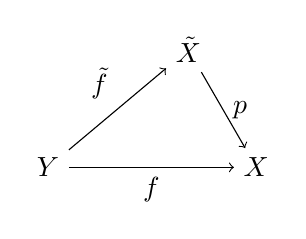
\begin{tikzpicture}[scale=1.15]
  \node (Y)  at (0,0)     {$Y$};
  \node (X)  at (2.3,0)   {$X$};
  \node (Xt) at (1.55,1.3) {$\tilde X$};
  \draw[->] (Y) -- node[below] {$f$} (X);
  \draw[->] (Y) -- node[above left] {$\tilde f$} (Xt);
  \draw[->] (Xt) -- node[right] {$p$} (X);
\end{tikzpicture}
\end{center}
\end{definition}

\Fig[0.62\linewidth]{figures/fig_2_1.png}{2.1}{实直线作为圆周的覆叠空间。}

特别有趣的是道路提升的存在性。这导致 $X$ 与 $\tilde X$ 的基本群之间的联系。

\begin{proposition}[2.4]
设 $f\colon I\to X$ 为端点是 $f(0)=x$ 与 $f(1)=y$ 的道路。对每个 $\tilde x\in p^{-1}(x)$，存在唯一的提升 $\tilde f\colon I\to\tilde X$，满足 $\tilde f(0)=\tilde x$ 且 $p\circ\tilde f=f$。
\end{proposition}

\begin{proof}
取 $X$ 的一个开覆盖 $\{U_a\}$，使得每个开集 $U_a$ 都是覆叠邻域。对每个 $s\in I$ 存在 $s$ 的邻域 $V_s$，使得 $f(V_s)\subset U_a$（对某个 $a$）。于是 $\{V_s\mid s\in I\}$ 是 $I$ 的开覆盖。但 $I$ 紧，由 Lebesgue 引理，存在 $\epsilon>0$，使得当 $|s-t|\le\epsilon$ 时 $f([s,t])\subset U_a$（对某个 $a$）。现在取 $n\in\N$ 使得 $\tfrac{1}{n}<\epsilon$，并令 $s_k=\tfrac{k}{n}$。不妨设 $f(0)\in U_a$。

定义 $\tilde f(0)=\tilde x\in U_a^i\subset p^{-1}(U_a)$，其中 $U_a^i$ 是互不相交的开集，且 $p|_{U_a^i}$ 是同胚。则对每个 $q\in[s_0,s_1]$，有 $f(q)\in U_a$，且 $p\colon U_a^i\to U_a$ 是同胚。我们现在可以定义
\[
\tilde f(q):=p^{-1}\bigl(f(q)\bigr),
\]
对每个 $q\in[s_0,s_1]$。由于 $[s_0,s_1]$ 连通，可知 $\tilde f([s_0,s_1])\subset U_a^i$，因而 $\tilde f|_{[s_0,s_1]}$ 唯一确定。现在通过迭代该过程把 $\tilde f$ 延拓到整个 $I$ 上。
\end{proof}

% [Tutor Note: Lebesgue 引理的正确表述是：紧度量空间 $I$ 的每个开覆盖有 Lebesgue 数 $\epsilon>0$，使直径 $<\epsilon$ 的任意子集都落在某个覆盖元素中。原文用 $|s-t|\le\epsilon$ 并写 $f([s,t])$，隐含 $s<t$。迭代延拓时还须保证每一步的起点落在同一片 $U_a^i$ 内，这由前一步的终点落在该片、且该片经 $p$ 同胚映到 $U_a$ 来保证。]

考虑基点 $x_0\in X$ 与 $\tilde x_0\in p^{-1}(x_0)\subset\tilde X$。

\begin{proposition}[2.5]
基本群上的诱导同态 $p_*\colon\pi_1(\tilde X,\tilde x_0)\to\pi_1(X,x_0)$ 是单射。此外，子群 $p_*\pi_1(\tilde X,\tilde x_0)$ 由以 $x_0$ 为基点且提升为以 $\tilde x_0$ 为基点的环路的那些环路组成。
\end{proposition}

\begin{proof}
对点 $[\tilde f_0]\in\ker(p_*)$，有 $\tilde f_0\colon I\to\tilde X$ 是以 $\tilde x_0$ 为基点的环路，且道路 $f_0=p\circ\tilde f_0$ 同伦于常值道路 $f_1(t)=x_0$（对每个 $t\in I$）。
% [原文 p.15]
对道路 $f_0$ 与 $f_1$ 之间的同伦 $f_t$，可以证明它提升为从 $\tilde f_0$ 到 $\tilde f_1$ 的唯一同伦 $\tilde f_t\colon I\to\tilde X$，满足 $p\circ\tilde f_t=f_t$。于是我们得到 $[\tilde f_0]=1$。
\end{proof}

\begin{proposition}[2.6]
覆叠 $p$ 的叶数等于子群 $p_*\bigl(\pi_1(\tilde X,\tilde x_0)\bigr)$ 在 $\pi_1(X,x_0)$ 中的指数。
\end{proposition}

\begin{proof}
先记 $H:=p_*\bigl(\pi_1(\tilde X,\tilde x_0)\bigr)$。对 $X$ 上以 $x_0$ 为基点的环路 $f$，考虑从右陪集到 $\{p^{-1}(x_0)\}$ 的映射 $\varphi\colon\{H[f]\}\to\{p^{-1}(x_0)\}$，满足 $\varphi(H[f])=\tilde f(1)$，其中 $\tilde f$ 是 $f$ 从点 $\tilde x_0$ 出发的提升。随后可以验证该映射 $\varphi$ 良定义、单射且满射。
\end{proof}

下一个定理对于拓扑空间覆叠空间的分类问题至关重要；我们首先引入如下技术术语：

\begin{definition}[2.7]
若拓扑空间 $X$ 对每个 $x\in X$ 都存在 $x$ 的邻域 $U$，使得同态 $i_*\colon\pi_1(U,x)\to\pi_1(X,x)$ 平凡，则称 $X$ 是\emph{半局部单连通的}。若对每个 $x\in X$ 和 $x$ 的每个邻域 $V$，都存在 $x$ 的邻域 $U\subset V$ 使得 $\pi_1(U,x)=\{e\}$ 平凡，则称 $X$ 是\emph{局部单连通的}。
\end{definition}

\Fig[0.70\linewidth]{figures/fig_2_2.png}{2.2}{夏威夷耳环（左）及其上的锥（右）。}

由
\[
H=\bigcup_{n=1}^{\infty}\Bigl\{(x,y)\in\R^2\ \Big|\ \Bigl(x-\frac{1}{n}\Bigr)^2+y^2=\frac{1}{n^2}\Bigr\}
\]
定义的拓扑空间被称为\emph{夏威夷耳环}；它展示在图 2.2 的左侧。它是非半局部单连通拓扑空间的一个标准例子：$(0,0)$ 的任意邻域都包含无穷多个圆周，从而包含其中的不可缩环路，而这些环路在 $H$ 中仍然不可缩。夏威夷耳环上的锥展示在同一图的右侧；它是一个半局部单连通但非局部单连通的拓扑空间的例子。

% [Tutor Note: “半局部单连通”与“局部单连通”不可混淆。锥 $CH$ 是半局部单连通的：$CH$ 可缩，故 $\pi_1(CH,x)=0$，“同态平凡”自动成立；但它在锥点处不局部单连通（锥点的任意小邻域都含绕锥点的非平凡环路）。核对夏威夷耳环非半局部单连通：任意 $\epsilon$-球内包含无穷多个圆 $(x-\frac1n)^2+y^2=\frac1{n^2}$，且这些小圆在 $H$ 中的同伦类非平凡。]

% [原文 p.16]
\begin{theorem}[2.8]
设 $X$ 是道路连通、局部道路连通且半局部单连通的拓扑空间。则存在 $X$ 的覆叠空间 $\tilde X$，使得 $\pi_1(\tilde X)=1$。空间 $\tilde X$ 称为 $X$ 的\emph{万有覆叠空间}。
\end{theorem}

\begin{remark}[2.9]
在本书后续部分，我们将只关注满足上述定理条件的拓扑流形。因此，读者可以在此背景下理解该定理的陈述与证明。
\end{remark}

\begin{proof}[定理 2.8 的证明]
我们在此只勾勒主要想法；完整证明可参阅例如 [192, Sect. 1.3]。我们可以把 $\tilde X$ 的点视为 $X$ 的点的同伦类，即定义
\[
\tilde X=\bigl\{[\gamma]\ :\ \gamma \text{ 是 } X \text{ 上满足 } \gamma(0)=x_0 \text{ 的道路}\bigr\},
\]
并考虑映射 $p\colon\tilde X\to X$，$p([\gamma])=\gamma(1)$。由于假定 $X$ 道路连通，可推出映射 $p$ 是满射。

对 $x$ 的一个开道路连通邻域 $U$，使得映射 $\pi_1(U,x)\hookrightarrow\pi_1(X,x)$ 平凡，并且对满足 $\gamma(1)\in U$ 的道路 $\gamma$，我们现在可以考察子集族
\[
U_{[\gamma]}:=\bigl\{[\gamma\cdot\eta]\ :\ \eta \text{ 是 } U \text{ 上满足 } \eta(0)=\gamma(1) \text{ 的道路}\bigr\}.
\]
然后可以证明该集族 $U_{[\gamma]}$ 定义了 $\tilde X$ 上一个拓扑的开集基。关于这个拓扑，覆叠映射 $p\colon\tilde X\to X$ 是覆叠空间投影，最后验证 $\tilde X$ 道路连通且单连通。
\end{proof}

\begin{definition}[2.10]
设 $X$ 为道路连通的拓扑空间，$p_1\colon\tilde X_1\to X$、$p_2\colon\tilde X_2\to X$ 为 $X$ 的覆叠空间。若 $f$ 是同胚且 $p_1=p_2\circ f$，则称映射 $f\colon\tilde X_1\to\tilde X_2$ 为\emph{覆叠空间的同构}；若只有后一条件成立，则称 $f$ 为\emph{覆叠空间的同态}。此外，对 $X$ 的覆叠空间 $p\colon\tilde X\to X$，若 $f\colon\tilde X\to\tilde X$ 是覆叠空间的同构，则称 $f$ 为\emph{自同构}。
\end{definition}

覆叠空间的自同构构成一个群，它对我们在后文将要看到的内容具有核心重要性。

\begin{definition}[2.11]
设 $X$ 为道路连通的拓扑空间，$p\colon\tilde X\to X$ 为覆叠空间。自同构 $f\colon\tilde X\to\tilde X$ 称为\emph{覆叠变换}。在环路的拼接运算下，它们构成一个群，记作 $G(\tilde X)$。
\end{definition}

\begin{example}[2.12]
\begin{enumerate}
\item 令 $p\colon\R\to S^1$ 为如例 2.2 中 $p(x)=(\cos(2\pi x),\sin(2\pi x))$ 的单位圆周的覆叠空间，如图 2.1。该覆叠的覆叠变换是由 $x\mapsto x+n$（$n\in\Z$）给出的映射 $f_n\colon\R\to\R$。因此 $G(\tilde\R)\cong\Z$。
\item 令 $p\colon S^1\to S^1$ 为 $p(z)=z^n$（$n\in\Z$）的单位圆周的另一覆叠空间。此时 $G(\tilde{S^1})\cong\Z_n$。
\end{enumerate}
\end{example}

% [Tutor Note: 例 2.12 第 2 条中，$p(z)=z^n$ 要成为覆叠需 $n\ne0$；而 $G(\tilde{S^1})\cong\Z_n$ 的写法默认 $n>0$（$\Z_n$ 表示 $n$ 阶循环群）。核对：$n=2$ 时 $z\mapsto z^2$ 的覆叠变换是 $z\mapsto-z$，群阶为 $2$。]

% [原文 p.17]
注意作用 $G(\tilde X)\curvearrowright X$ 在连通空间 $\tilde X$ 上是\emph{覆叠空间作用}，即对任意点 $\tilde x\in\tilde X$、非平凡 $g\in G(\tilde X)$ 以及覆叠邻域 $\tilde U\ni\tilde x$，有 $g(\tilde U)\cap\tilde U=\varnothing$。特别地，若 $\tilde X$ 是万有覆叠空间，则由于 $G(\tilde X)=\pi_1(X,x_0)$，我们有 $\pi_1(X,x_0)\curvearrowright\tilde X$ 是覆叠空间作用。

% [Tutor Note: 原文此句写作 $G(\tilde X)\curvearrowright X$，目标空间漏了波浪号，应为 $G(\tilde X)\curvearrowright\tilde X$。依据是同句“on the connected space $\tilde X$”，以及紧接着的 $\pi_1(X,x_0)\curvearrowright\tilde X$ 也以 $\tilde X$ 为目标。]

\section{分歧覆叠}

我们在定义 2.1 中已经看到，两个拓扑空间之间的满射 $p\colon\tilde X\to X$ 若通过 $p$ 局部同胚，则为覆叠。这类覆叠实际上称为\emph{非分歧覆叠}。它对 $\tilde X$ 施加许多限制。分歧覆叠的概念灵活得多，它起源于复分析中多值函数的研究。在这些情形中，在底空间的孤立点上方，覆叠的叶可以合并，因此覆叠映射群可以有不动点。

\begin{example}[2.13]
考虑由 $f(z)=z^2$ 给出的映射 $f\colon\C\to\C$。限制到 $\C^*$ 上，它定义了 $2$ 叶覆叠。在原点处，两个叶合并。用下文定义的术语，我们将说原点是\emph{分支点}。
\end{example}

反函数 $z\mapsto\sqrt{z}$ 并非在整个 $\C$ 上良定义。有几种方式理解这个函数。若去掉从原点出发的一条射线（例如负实轴），则平方根是良定义的函数。也可以把 $\sqrt{z}$ 视为多值函数，对每个非零复数有两个值。还有一种方式是：$\sqrt{z}$ 不是 $\C$ 上的良定义函数，而是在由 $f$ 定义的分歧二重覆叠上的良定义函数。平方根的两个可能值分配给两个叶，而当你沿绕原点的环路行进时，就置换了两个叶。

现在我们把分歧覆叠的概念精确化：

\begin{definition}[2.14]
设 $X,\tilde X$ 为两个拓扑曲面。若存在非空离散集 $Y\subset X$，使得 $p|_{p^{-1}(X\setminus Y)}\colon p^{-1}(X\setminus Y)\to X\setminus Y$ 是定义 2.1 意义下的覆叠，则称连续满射 $p\colon\tilde X\to X$ 为（拓扑）\emph{分歧覆叠}。上述子集 $Y$ 称为 $p$ 的\emph{分支轨迹}，我们将把它记作 $B(p)$。点 $b\in Y$ 称为\emph{分支点}。
\end{definition}

我们进一步引入如下术语：

\begin{definition}[2.15]
设 $X,\tilde X$ 与 $p\colon\tilde X\to X$ 如上。考虑点 $\tilde x\in\tilde X$ 及其在 $p$ 下的像 $x:=p(\tilde x)$。映射 $p$ 在点 $\tilde x$ 处的\emph{分歧指数}定义为正整数 $m_{\tilde x}(p)$，使得存在 $\tilde x$ 的开邻域 $U$，点 $x\in X$ 在 $U$ 中只有一个原像，即 $p^{-1}(x)\cap U=\tilde x$，且对其余所有点 $z\in p(U)$ 都有 $|p^{-1}(z)\cap U|=m_{\tilde x}(p)$。若 $m_{\tilde x}(p)>1$，则称点 $\tilde x\in\tilde X$ 为 $\tilde X$ 的\emph{分歧点}。此时 $p(\tilde x)$ 是分支点。此外，映射 $p$ 的\emph{分歧轨迹} $R(p)$ 是 $\tilde X$ 中由所有分歧点构成的子集；另见图 2.3 的例子。
\end{definition}

% [Tutor Note: 定义 2.15 中 $p^{-1}(x)\cap U=\tilde x$ 严格应写作 $p^{-1}(x)\cap U=\{\tilde x\}$：原文把单点集与其元素等同，属记号滥用，引述时勿照抄成集合恒等式。]

% [原文 p.18]
\Fig[0.72\linewidth]{figures/fig_2_3.png}{2.3}{映射 $p\colon\tilde X\to X$ 有两个分支点 $x_1,x_2\in X$ 与两个分歧点 $\tilde x_1,\tilde x_2\in\tilde X$。注意这里 $m_{\tilde x_1}(p)=3$，$m_{\tilde x_2}(p)=2$。}

鉴于上述定义，总有 $R(p)\subseteq p^{-1}(B(p))$。此外，只要 $R(p)=\varnothing$，映射 $p$ 就是非分歧覆叠。当所有分支点的指数为 $2$ 时，我们称之为\emph{简单分歧覆叠}。对每个点 $x\in X$，我们现在考虑映射 $p$ 在各原像处的分歧指数之和：
\[
d_x(p):=\sum_{\tilde x\in p^{-1}(x)}m_{\tilde x}(p).
\]
数 $d_x(p)$ 实际上对一切 $x\in X$ 的点都是常数（证明见 [269, Chap. II, Prop. 4.8]）。于是引出如下定义：

\begin{definition}[2.16]
设 $X,\tilde X$ 与 $p\colon\tilde X\to X$ 如上。映射 $p$ 的\emph{次数}是对任意点 $x\in X$ 的整数 $d_x(p)$，因此将简记为 $\deg(p)$。
\end{definition}

下面的例子给出黎曼曲面上分歧覆叠的局部模型，特别是我们将在 §8.4 进一步讨论的谱曲线。

\begin{example}[2.17]
考虑开集 $U\subset\C$ 与平凡丛 $E=U\times\C$。用 $z$ 表示 $U$ 上的坐标，$p$ 表示纤维上的坐标。对全纯函数 $a_2(z),a_3(z),\dots,a_n(z)$，定义函数
\[
P(p,z)=p^n+a_2(z)p^{n-2}+a_3(z)p^{n-3}+\cdots+a_n(z),
\]
它是 $p$ 的多项式。最后考虑
\[
\tilde U=\{(z,p)\in E\mid P(p,z)=0\}.
\]
把典范投影 $E\to U$ 限制到 $\tilde U$，我们得到覆叠 $\pi\colon\tilde U\to U$，它在多项式 $P$ 的重零点处分歧。$\pi$ 的次数为 $n$，即 $P$ 作为 $p$ 的多项式的次数。若 $P$ 至多有二重零点，则该覆叠是简单分歧的。
\end{example}

% [Tutor Note: 例 2.17 的多项式 $P$ 缺 $p^{n-1}$ 项（其系数取 $0$），这不是笔误：这正是 $\SL_n$ 谱曲线（迹零）的标准形式，与 §8.4 及后文 Hitchin 系统的约定一致；若按一般 $n$ 次多项式补上 $a_1(z)p^{n-1}$，得到的将是 $\GL_n$ 型的谱覆盖。核对方式：$n=2$ 时 $P=p^2+a_2(z)$，对应迹为零的二阶谱曲线。]

现在我们准备陈述拓扑曲面情形下的基本 \emph{Riemann--Hurwitz 公式}：

% [原文 p.19]
\begin{theorem}[2.18]
（Riemann--Hurwitz 公式）设 $S_{g_1,h_1},S_{g_2,h_2}$ 是一对紧连通可定向拓扑曲面，亏格分别为 $g_1$ 与 $g_2$，边界分支数分别为 $h_1$ 与 $h_2$。设 $p\colon S_{g_1,h_1}\to S_{g_2,h_2}$ 为（可能分歧的）拓扑曲面覆叠。则
\[
2g_1+h_1-2=\deg(p)\bigl(2g_2+h_2-2\bigr)+\sum_{x\in S_{g_1,h_1}}\bigl(m_x(p)-1\bigr).
\]
\end{theorem}

证明的想法是：考虑 $S_{g_2,h_2}$ 的一个与分支点相适应的三角剖分（即所有分支点都作为三角剖分的顶点出现），并取它在 $p$ 下的原像，得到 $S_{g_1,h_1}$ 上的一个三角剖分。然后用 Euler 公式 $\chi(S_{g_1,h_1})=V-E+F$ 计算 $S_{g_1,h_1}$ 的 Euler 示性数，其中 $V,E,F$ 分别是 $S_{g_1,h_1}$ 上三角剖分的顶点数、边数与面数。完整证明参见 [269, Chap. II, Prop. 4.16]。

Riemann--Hurwitz 公式是一个强大的工具，应用极多。它的起源可追溯到黎曼曲面的研究，我们将在 §3.1 更仔细地介绍黎曼曲面。黎曼曲面是连通的 $1$ 维复流形；假设黎曼曲面之间的覆叠映射 $p\colon S_{g_1,h_1}\to S_{g_2,h_2}$ 是复解析的，则 $p$ 在点 $x\in S_{g_1,h_1}$ 处分歧，当且仅当 $p$ 在 $x$ 附近的局部坐标 $z$ 下局部表示为 $p(z)=z^n$（对某个整数 $n>1$）。这个数 $n$ 就是点 $x\in S_{g_1,h_1}$ 处的分歧指数。

% [Tutor Note: 可用 $p(z)=z^n\colon\PP^1\to\PP^1$ 核对公式：$g_1=g_2=0$、$h_1=h_2=0$，分支点为 $0$ 与 $\infty$，两处 $m=n$，右端 $=n(-2)+2(n-1)=-2=$ 左端。还须注意求和指标写在上曲面 $S_{g_1,h_1}$ 上（与定义 2.15 的 $m_{\tilde x}$ 一致）；若误改成对底曲面求和，会漏掉分歧贡献。]

除了在本专著的第 II 部分与第 III 部分中的作用之外，分歧覆叠与黎曼曲面还将在第 21、22 章中显著出现，那里将讨论 S 类理论及其 BPS 态。

% [原文 p.20]
% 原文此页为空白页（第 2 章结束后的空白页），无正文。
